%%%%%%%%%%%%%%%%%%%%%%%%%%%%%%%%%%%%%%%%%
% Beamer Presentation
% LaTeX Template
% Version 1.0 (10/11/12)
%
% This template has been downloaded from:
% http://www.LaTeXTemplates.com
%
% License:
% CC BY-NC-SA 3.0 (http://creativecommons.org/licenses/by-nc-sa/3.0/)
%
%%%%%%%%%%%%%%%%%%%%%%%%%%%%%%%%%%%%%%%%%

%----------------------------------------------------------------------------------------
%	PACKAGES AND THEMES
%----------------------------------------------------------------------------------------

\documentclass{beamer}

\mode<presentation> {

% The Beamer class comes with a number of default slide themes
% which change the colors and layouts of slides. Below this is a list
% of all the themes, uncomment each in turn to see what they look like.

%\usetheme{default}
%\usetheme{AnnArbor}
%*\usetheme{Antibes}
%\usetheme{Bergen}
%*\usetheme{Berkeley}
\usetheme{Berlin}
%\usetheme{Boadilla}
%\usetheme{CambridgeUS}
%\usetheme{Copenhagen}
%\usetheme{Darmstadt}
%\usetheme{Dresden}
%\usetheme{Frankfurt}
%\usetheme{Goettingen}
%\usetheme{Hannover}
%\usetheme{Ilmenau}
%\usetheme{JuanLesPins}
%\usetheme{Luebeck}
%\usetheme{Madrid}
%\usetheme{Malmoe}
%\usetheme{Marburg}
%\usetheme{Montpellier}
%\usetheme{PaloAlto}
%\usetheme{Pittsburgh}
%\usetheme{Rochester}
%\usetheme{Singapore}
%\usetheme{Szeged}
%\usetheme{Warsaw}

% As well as themes, the Beamer class has a number of color themes
% for any slide theme. Uncomment each of these in turn to see how it
% changes the colors of your current slide theme.

%\usecolortheme{albatross}
%\usecolortheme{beaver}
%\usecolortheme{beetle}
%\usecolortheme{crane}
%\usecolortheme{dolphin}
%\usecolortheme{dove}
%\usecolortheme{fly}
%\usecolortheme{lily}
%\usecolortheme{orchid}
%\usecolortheme{rose}
%\usecolortheme{seagull}
%\usecolortheme{seahorse}
%\usecolortheme{whale}
%\usecolortheme{wolverine}

%\setbeamertemplate{footline} % To remove the footer line in all slides uncomment this line
%\setbeamertemplate{footline}[page number] % To replace the footer line in all slides with a simple slide count uncomment this line

%\setbeamertemplate{navigation symbols}{} % To remove the navigation symbols from the bottom of all slides uncomment this line
}

\usepackage[utf8]{inputenc}
\usepackage{graphicx} % Allows including images
\usepackage{booktabs} % Allows the use of \toprule, \midrule and \bottomrule in tables

%----------------------------------------------------------------------------------------
%	TITLE PAGE
%----------------------------------------------------------------------------------------

\AtBeginSection[]{
	\begin{frame}
	\vfill
	\centering
	\begin{beamercolorbox}[sep=8pt,center,shadow=true,rounded=true]{title}
		\usebeamerfont{title}\insertsectionhead\par%
	\end{beamercolorbox}
	\vfill
\end{frame}
}

\definecolor{purple}{RGB}{127,0,255}

\title[Redes de visibilidad]{Sistemas de monitorización de latencias en redes de visibilidad} % The short title appears at the bottom of every slide, the full title is only on the title page

\author{J. Álvaro Garrido López} % Your name
\institute[UGR] % Your institution as it will appear on the bottom of every slide, may be shorthand to save space
{
Universidad de Granada \\ % Your institution for the title page
\medskip
Tutores: Javier Díaz y Miguel Jiménez\\
\medskip
Trabajo de Fin de Grado\\
}
\date{\today} % Date, can be changed to a custom date

\begin{document}

\begin{frame}
\titlepage % Print the title page as the first slide
\end{frame}

\begin{frame}
\frametitle{Índice} % Table of contents slide, comment this block out to remove it
\tableofcontents % Throughout your presentation, if you choose to use \section{} and \subsection{} commands, these will automatically be printed on this slide as an overview of your presentation
\end{frame}

%----------------------------------------------------------------------------------------
%	PRESENTATION SLIDES
%----------------------------------------------------------------------------------------

%------------------------------------------------
%\section{First Section} % Sections can be created in order to organize your presentation into discrete blocks, all sections and subsections are automatically printed in the table of contents as an overview of the talk
%------------------------------------------------

%\subsection{Subsection Example} % A subsection can be created just before a set of slides with a common theme to further break down your presentation into chunks

%------------------------------------------------
\section{Introducción}
%------------------------------------------------

\begin{frame}
\frametitle{Redes de visibilidad y aplicaciones}
\begin{block}{¿Qué son las redes de visibilidad?}
	Son la infraestructura en una red que permite la monitorización de la misma, con el fin de conocer el estado sobre su rendimiento y de detectar posibles fallos de seguridad.
\end{block}

\begin{figure}[H]
	\centering
	
\includegraphics[scale=0.3]{garland3.jpeg}
	\label{garland2}
\end{figure}

\end{frame}

%------------------------------------------------

\begin{frame}
\frametitle{Redes de visibilidad y aplicaciones}

\begin{figure}[H]
	\centering
	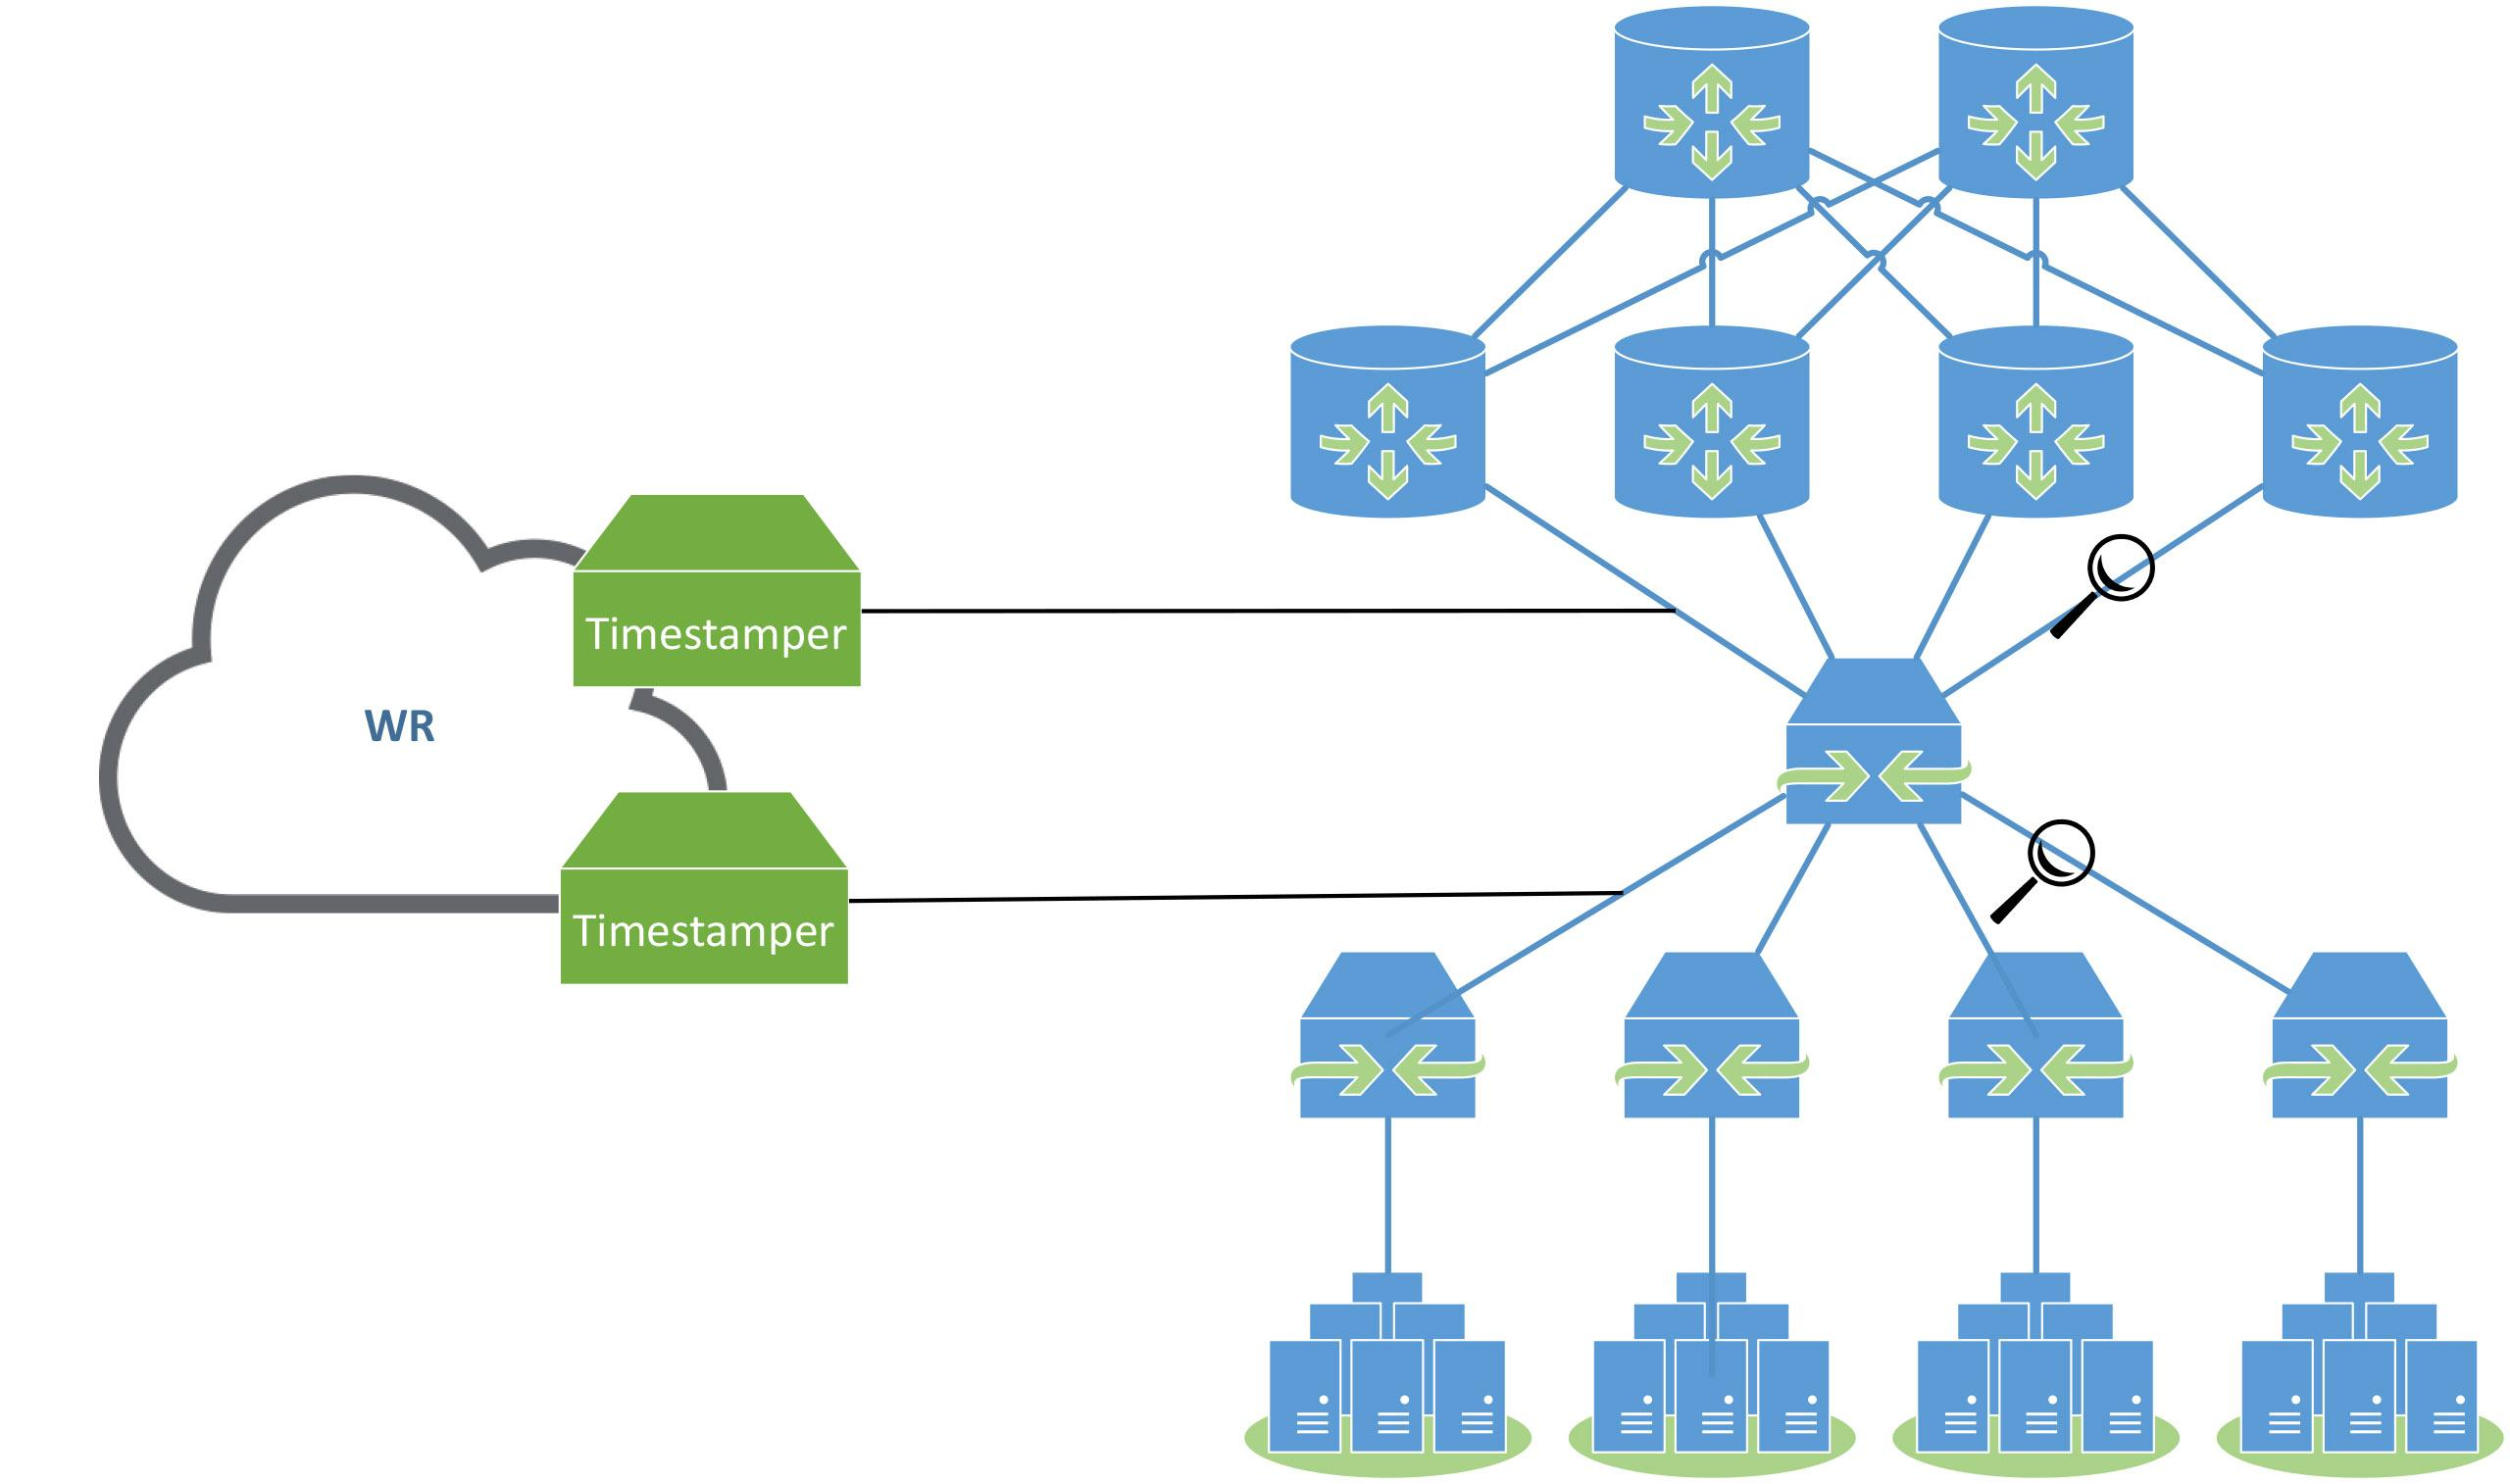
\includegraphics[scale=0.1]{visibility.jpg}
	\label{visibility}
\end{figure}

\end{frame}

%------------------------------------------------

\begin{frame}
\frametitle{Motivación y contexto}
\begin{block}{Contexto}
\begin{itemize}
	\item Volúmenes ingentes de datos
	\item Preocupación por la seguridad
	\item Servicios de altas prestaciones (telecom y finance)
	\item Necesidad de controlar constante y eficientemente el tráfico
	\item Auge del \textit{Big Data}
\end{itemize}
\end{block}

\begin{itemize}
	\item Ingredientes perfectos para que se requiera de una recopilación, distribución y entrega de datos eficaz y escalable.
	\item De este punto parte la \textbf{visibilidad en redes}.
\end{itemize}

\end{frame}

\begin{frame}
\frametitle{Objetivos (I)}

\begin{itemize}
	\item Estado de la técnica sobre captura eficiente
	\item Aplicaciones comerciales y libres para visibilidad
	\item Análisis sobre las características de las tecnologías encontradas
	\item Evaluación del funcionamiento lógico de tecnologías
\end{itemize}

\end{frame}

\begin{frame}
\frametitle{Objetivos (II)}
\begin{itemize}
	\item Diseño y desarrollo del sistema. Favorecer escalabilidad y flexibilidad
	\item Integración de los componentes \textit{hardware} y \textit{software}
	\item Integración de un sistema de alerting
\end{itemize}

\end{frame}

%------------------------------------------------

\begin{frame}
\frametitle{Material y métodos}

\begin{figure}[H]
	\centering
	
\includegraphics[scale=0.30]{material.png}
	\label{material}
\end{figure}

\end{frame}

%------------------------------------------------
\section{Estado de la técnica}
%------------------------------------------------

%------------------------------------------------

\begin{frame}

\frametitle{Métodos para implementar visibilidad (I)}
\begin{itemize}
	\item Mediante peticiones \textbf{SNMP}
	\item A través de \textbf{gestión directa} del tráfico (e.g. mediante \textbf{TAP})
	\item Gestión del tráfico \textbf{por flujos} (e.g. \textbf{sflow})
\end{itemize}

\end{frame}

\begin{frame}
\frametitle{Métodos para implementar visibilidad (II). Gestión directa}

\begin{figure}[H]
	\centering
	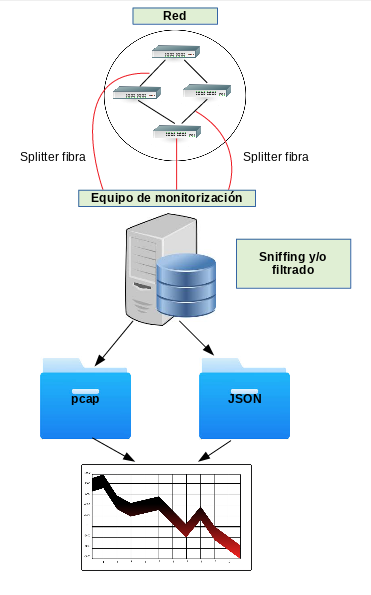
\includegraphics[scale=0.35]{directo.png}
	\label{directo}
\end{figure}

\end{frame}

\begin{frame}
\frametitle{Métodos para implementar visibilidad (III). Gestión por flujos}

\begin{figure}[H]
	\centering
	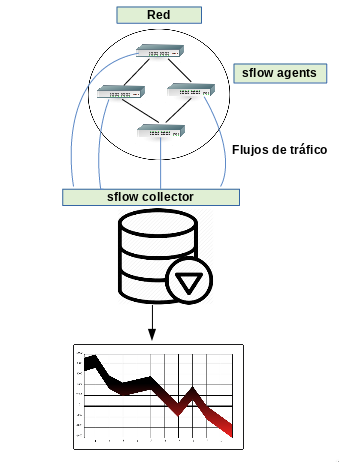
\includegraphics[scale=0.5]{sflow.png}
	\label{sflow}
\end{figure}

\end{frame}

\begin{frame}

\frametitle{\textit{Hardware} específico para visibilidad (I)}

\begin{itemize}
	\item \textbf{Divisores ópticos}. Dividen el haz de luz en varios caminos. No consumen electricidad
	\item \textbf{SPAN}. Puerto en un \textit{switch} a donde se replica el tráfico. Existe pérdida de paquetes
	\item \textbf{\color{purple}{TAP}}. Replican el tráfico asegurando 0 pérdida de paquetes
	\item \textbf{Agregadores}. Agregan el flujo de tráfico de diferentes puertos en uno escogido
\end{itemize}

\end{frame}

\begin{frame}
\frametitle{\textit{Hardware} específico para visibilidad (II)}

\begin{figure}[H]
	\centering
	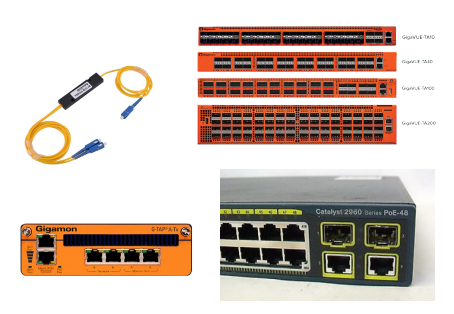
\includegraphics[scale=0.7]{hardware.png}
	\label{hardware}
\end{figure}

\end{frame}

%------------------------------------------------
\section{Implementación}
%------------------------------------------------

%------------------------------------------------

\begin{frame}
\frametitle{Pruebas preliminares (I)}

\textbf{Gestión del tráfico basado en flujos}

\begin{block}{¿Qué es un flujo?}
	Es una secuencia de paquetes que comparten las mismas propiedades que son enviados entre un \textit{host} emisor y un receptor. Por ejemplo, en una emisión de \textit{streaming}, los paquetes son enviados por el servidor forman parte del mismo flujo. 
\end{block}

\end{frame}

\begin{frame}
\frametitle{Pruebas preliminares (II)}

\textbf{Tecnologías existentes}

\begin{itemize}
	\item \textbf{NetFlow}. Propietaria de \textbf{CISCO}. Necesario exportar flujos cada cierto tiempo
	\item \textbf{\color{purple}{sflow}}. Tecnología compatible con múltiples fabricantes. Datagramas enviados en tiempo real. Más recomendado para visibilidad
\end{itemize}

A pesar de escoger \textbf{sflow} por su mayor compatibilidad, y comprobar sus virtudes, nos interesa la opción más escalable y versátil. Por tanto, descartamos trabajar con gestión del tráfico por flujos.

\end{frame}

%------------------------------------------------

\begin{frame}
\frametitle{Captura de paquetes}

\begin{itemize}
	\item \textbf{libpcap}. Biblioteca por defecto en Linux. Búffer lineal. Tamaño reducido
	\item \textbf{\color{purple}{pf\_ring ZC}}. Búffer circular con \textbf{DMA}
	\item \textbf{Sniffer 10G}. Tecnología propietaria 10G. Depende de \textit{hardware} específico del fabricante.
\end{itemize}

Escogemos \textbf{pf\_ring} por ser mayoritariamente de código abierto, versátil, y no depender de \textit{hardware} específico.

\end{frame}

%------------------------------------------------

\begin{frame}[fragile] % Need to use the fragile option when verbatim is used in the slide
\frametitle{Filtrado}

\begin{itemize}
	\item \textbf{Hardware}. Existen \textbf{NIC} que ofrecen la posibilidad de aplicar reglas de filtrado \textit{hw}
	\item \textbf{Bloque IP en FPGA}. También existe la posibilidad de implementar un bloque IP en una FPGA para el filtrado
	\item \textbf{\color{purple}{Software}}. \textbf{BPF} es una biblioteca que permite el filtrado \textit{software} haciendo uso de cualquier herramienta de captura que hayamos escogido anteriormente
\end{itemize}

No escogemos la opción \textit{hardware} por la limitación de compatibilidad, tampoco la opción de implementar un bloque IP por la complejidad de la solución.\\
Entonces, la más escalable es la opción \textit{software}

\end{frame}

%------------------------------------------------

\begin{frame}
\frametitle{Almacenamiento}

\begin{itemize}
	\item \textbf{InfluxDB}. Base de datos rendimiento \textit{real-time}. Escalabilidad buena
	\item \textbf{elasticsearch}. Base de datos rendimiento \textit{near real-time}. Alta flexibilidad del \textit{input} y \textit{output} de datos haciendo uso del \textit{stack ELK}
\end{itemize}

Escogemos \textit{elasticsearch} por su flexibilidad y escalabilidad apoyándose en el \textit{stack ELK}

\end{frame}

%------------------------------------------------

\begin{frame}
\frametitle{Visibilidad}

\begin{itemize}
	\item \textbf{Grafana}. Escalabilidad buena. Diferentes opciones para visualizar parámetros
	\item \textbf{\color{purple}{Kibana}}. Gran escalabilidad. Compatibilidad con \textit{JSON}. Apoyo en \textit{stack ELK}. Tratamiento previo de los datos con \textit{Logstash}
	\item \textbf{Graphite}. Buena compatibilidad y escalabilidad
\end{itemize}

Nos quedamos con \textbf{Kibana} por haber demostrado ser la opción más escalable por su compatibilidad y flexibilidad con \textit{JSON}, por las etapas previas y tratamiento de datos con \textit{Logstash}, y por la multitud de opciones para visualización que ofrece

\end{frame}

%------------------------------------------------

\begin{frame}
\frametitle{Setup final}

\begin{figure}[H]
	\centering
	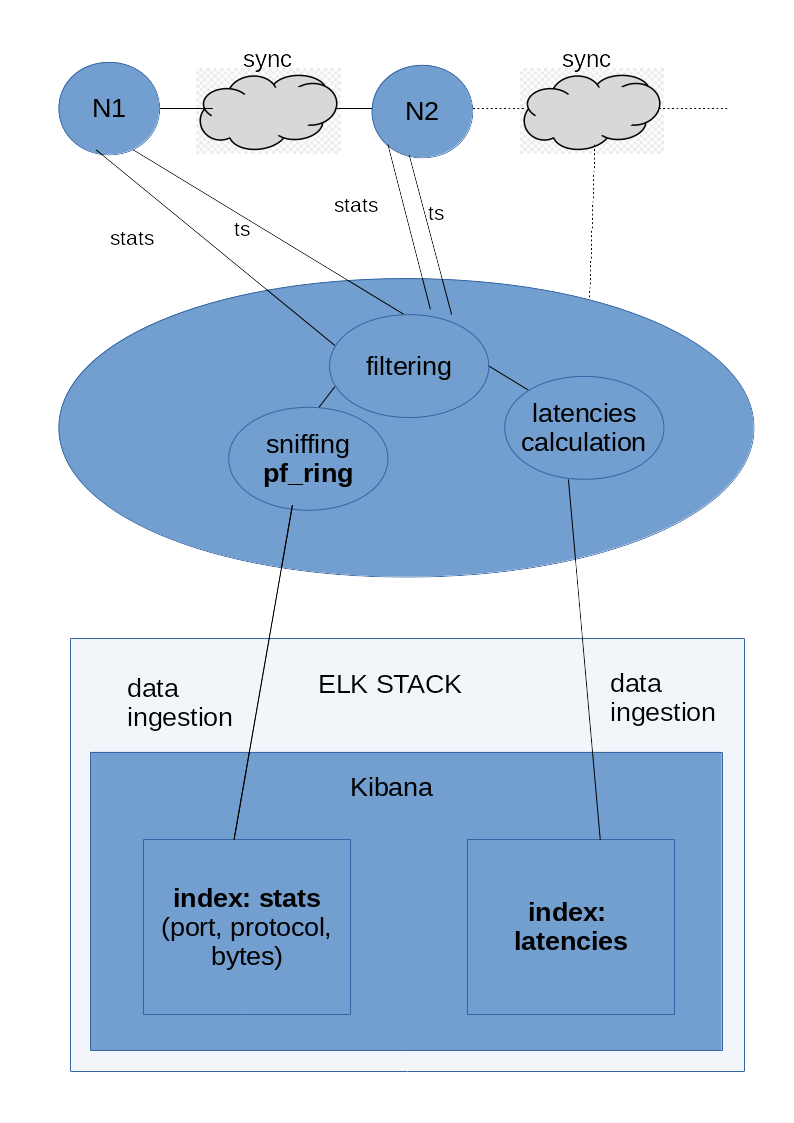
\includegraphics[scale=0.2]{sistema-final.png}
	\label{sistema-final}
\end{figure}

\end{frame}

%------------------------------------------------
\section{Resultados}
%------------------------------------------------

%------------------------------------------------

\begin{frame}
\frametitle{Visualización de estadísticas (I)}

\begin{figure}[H]
	\centering
	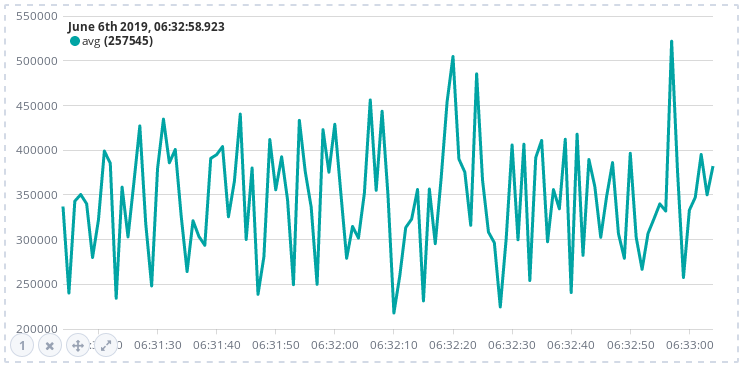
\includegraphics[scale=0.5]{timelion-avg.png}
	\label{timelionavg}
\end{figure}

\end{frame}

%------------------------------------------------

\begin{frame}
\frametitle{Visualización de estadísticas (II)}

\begin{figure}[H]
	\centering
	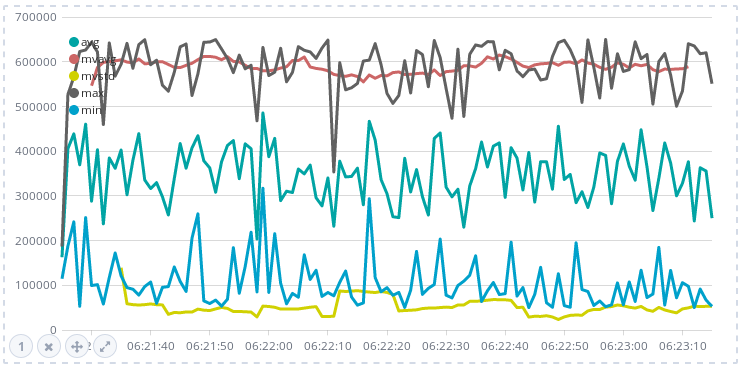
\includegraphics[scale=0.5]{timelion-all-stats.png}
	\label{timelion}
\end{figure}

\end{frame}

%------------------------------------------------

\begin{frame}
\frametitle{Comparativa captura de paquetes (I). libpcap}

\begin{figure}[H]
	\centering
	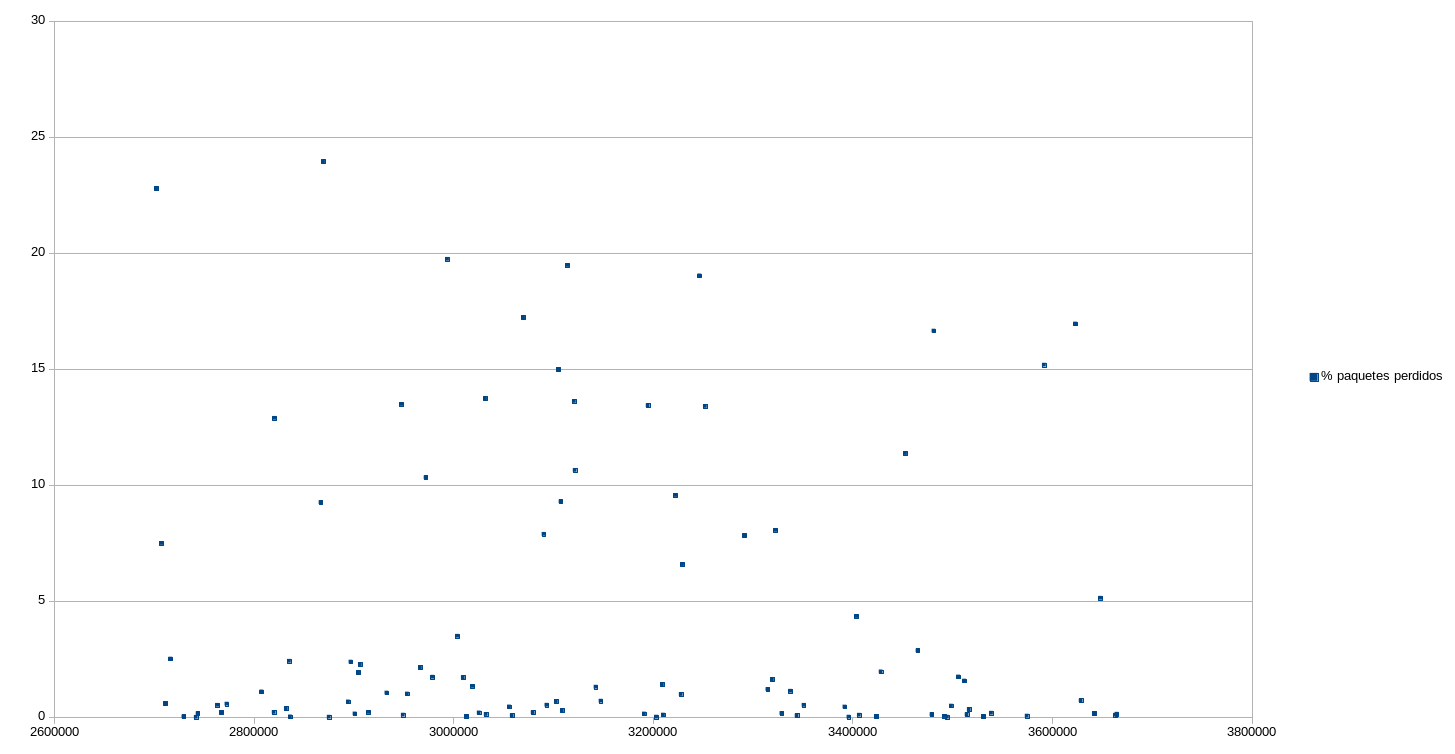
\includegraphics[scale=0.25]{captura-libpcap-original.png}
	\label{libpcap}
\end{figure}

\end{frame}

\begin{frame}
\frametitle{Comparativa captura de paquetes (II). pf\_ring}

\begin{figure}[H]
	\centering
	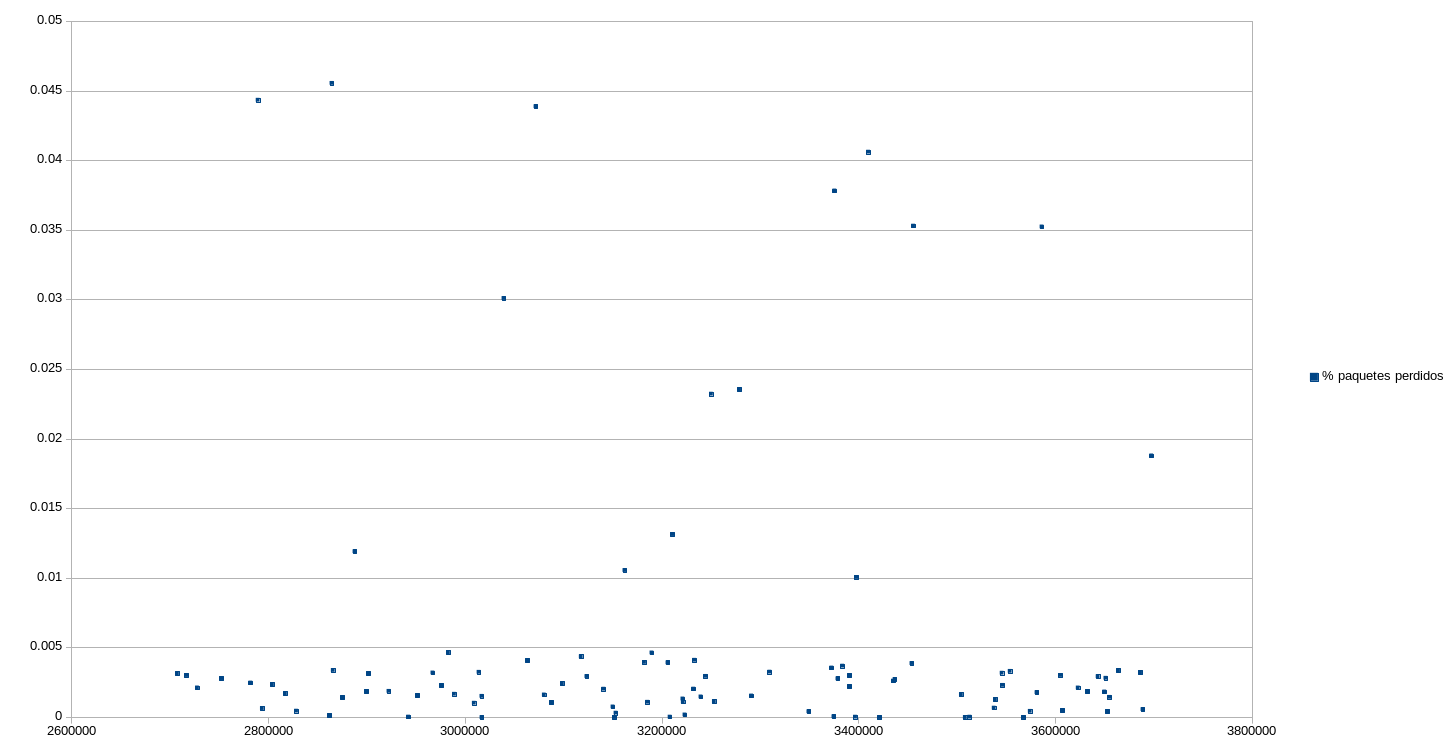
\includegraphics[scale=0.25]{captura-libpcap-aware-pfring.png}
	\label{pfring}
\end{figure}

\end{frame}

%------------------------------------------------
\section{Conclusiones}
%------------------------------------------------

%------------------------------------------------

\begin{frame}
\frametitle{Conclusiones}
Hemos construido una herramienta que:

\begin{itemize}
	\item Integra soluciones a diferentes niveles para construir una herramienta para medir latencias y otras estadísticas
	\item Es posible sustituir componentes de la misma para satisfacer necesidades más específicas, por la \textbf{alta escalabilidad} y \textbf{flexibilidad} del sistema
	\item Mejora de hasta un 30\% en la etapa de captura de paquetes (pf\_ring) sobre \textit{libpcap})
	\item Permite implementar visibilidad en una red
	\item Permite mucho trabajo futuro
	\item Ya tiene asignada una futura \textbf{aplicación} en el mercado (Seven)
\end{itemize}

\end{frame}

%------------------------------------------------

\begin{frame}
\frametitle{Trabajo futuro}
\begin{itemize}
	\item Apoyo \textit{hardware} para filtrado (FPGA)
	\item Creación de campos para medición de latencias con mayor precisión
	\item Data Analytics / Big Data
\end{itemize}

\end{frame}

%------------------------------------------------

\begin{frame}
\frametitle{Referencias}
\footnotesize{
\begin{thebibliography}{99} % Beamer does not support BibTeX so references must be inserted manually as below
%\bibitem[Smith, 2012]{p1} John Smith (2012)
%\newblock Title of the publication
%\newblock \emph{Journal Name} 12(3), 45 -- 678.
\bibitem{seven} Seven Solutions website (2019)
\newblock \url{https://sevensols.com/index.php/visibility-network/}
\bibitem{garland} Garland Technology (2019)
\newblock \url{https://www.garlandtechnology.com/}
\bibitem{gigamon} Gigamon (2019)
\newblock \url{https://www.gigamon.com/products/access-traffic/network-taps.html}
\end{thebibliography}
}
\end{frame}

%----------------------------------------------------------------------------------------

\end{document} 